\chapter{Análisis de conjunto de datos transcripcionales de respuesta a stress abiótico en plantas}
En este capítulo analizaremos el conjunto de datos transcripcionales obtenidos por Wiegel \& Lohmann para la planta Arabidopsis thaliana presentados en la sección \ref{sec:wiegel}, utilizando para ello los métodos de agrupamiento k-means (sección \ref{sec:agrupamientos_no_jerarquicos}) y corte de árbol dinámico híbrido (sección \ref{sec:grupos_en_agrupamiento_jerarquico}) introducidos en el capítulo \ref{materiales_y_metodos}.\\\\
Una vez obtenidos los grupos en el espacio de expresión, utilizaremos índices BHI e Interacting Densities para cuantificar el grado de coherencia entre estas estructuras y el conocimiento almacenado en el espacio GO.\\\\
Luego, analizaremos la coherencia de los resultados obtenidos en el espacio de expresión con la de resultados obtenidos en otros espacios de conocimiento, como GO (sección \ref{sec:go}), PIN  (sección \ref{sec:redes}) y KEGG (sección \ref{sec:kegg}), esperando que estos conocimientos sean diferentes pero no ortogonales. 

\section{Proceso de filtrado}
El conjunto de datos transcripcionales utilizado consta de los niveles de expresión de 22810 sondas que se mapean a 20149 genes a lo largo de 11 tratamientos diferentes y con entre 4 y 9 puntos muestreados por duplicado. Para comenzar nuestro análisis realizamos un proceso de filtrado no-especifico de manera de focalizarnos en aquellos genes que estuvieran en principio siendo regulados a lo largo del experimento.\\\\
Para ello, se aplicaron dos tipos de filtros por tratamiento. Para el primero, se calculó la desviación estándar por gen a lo largo de todo el tratamiento y se decidió tomar los genes cuya desviación estándar se encontrara en el cuantil 0.9, es decir, utilizar el 10\% de los genes con mayor desviación estándar, considerando estos como los que forman parte de la respuesta biológica al tratamiento. La figura \ref{fig:densidad_de_desviacion_estandar} muestra la distribución de probabilidad acumulada (empírica) de la desviación estándar para los genes del tratamiento ``Frío''.\\\\
Una vez aplicado este filtro por desviación estándar, se aplicó un filtro de tipo ``$K sobre A$'', que conserva únicamente aquellos genes que tengan al menos $K$ datos por encima del valor $A$. En nuestro caso, decidimos utilizar como valor de $K$, la mitad de las mediciones que tuviera el tratamiento. Si el tratamiento tenía mediciones a los 0 minutos, 30 minutos, 1 hora, 3 horas, 6 horas, 12 horas y 24, es decir, 6 mediciones en total, se tomó $K = 3$. Para $A$, se decidió utilizar una medida de $A=4$. Analizando la distribución bimodal de la figura \ref{fig:densidad_para_niveles} vemos que este valor permite descartar casos posiblemente asociados a un nivel de fondo de expresión.
\begin{figure*}[t!]
    \centering
    \begin{subfigure}[t]{0.45\textwidth}
    \centering
    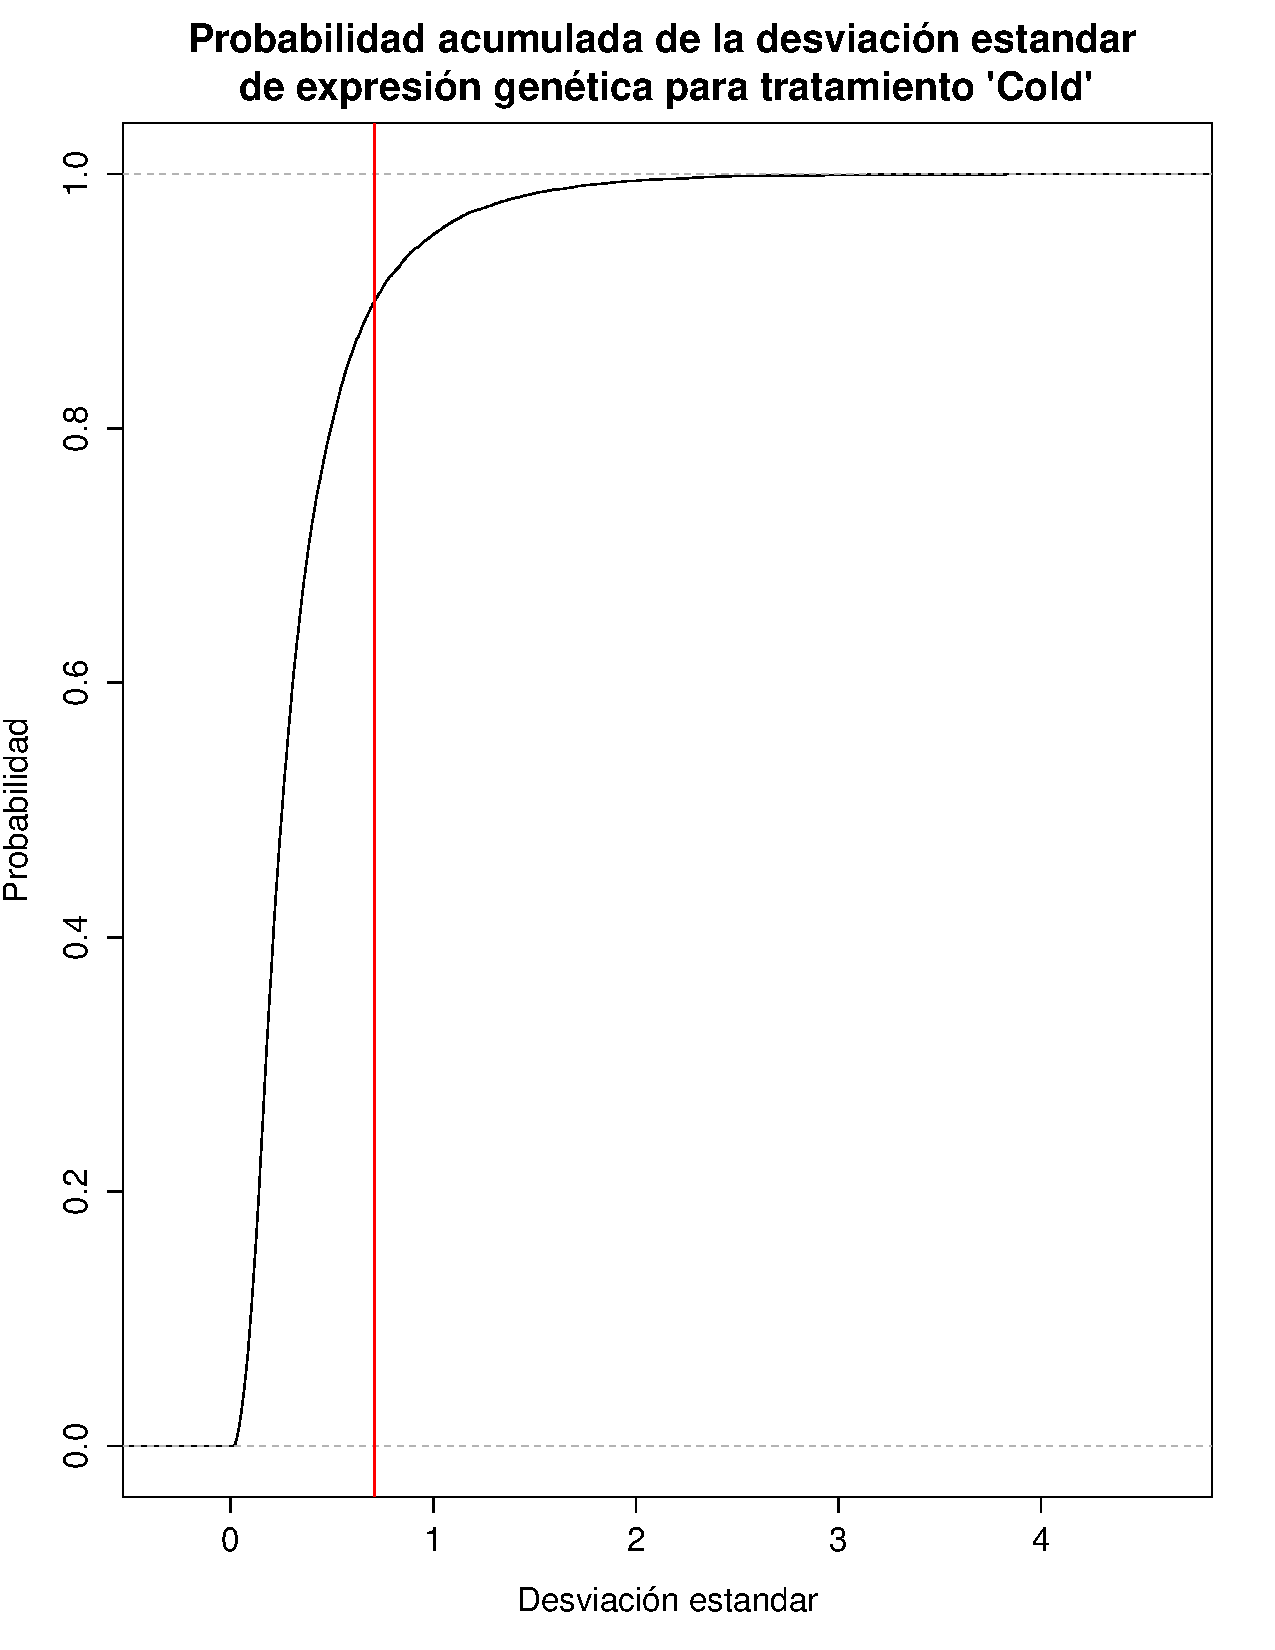
\includegraphics[width=1\textwidth]{densidad_de_desviacion_estandar.pdf}
    \caption{Distribución de probabilidad acumulada de la desviación estándar para los genes del tratamiento 'Frío'. Todos los genes con desviación estándar menor que la indicada por la recta vertical roja son descartados.}
    \label{fig:densidad_de_desviacion_estandar}
    \end{subfigure}
    \begin{subfigure}[t]{0.45\textwidth}
    \centering
    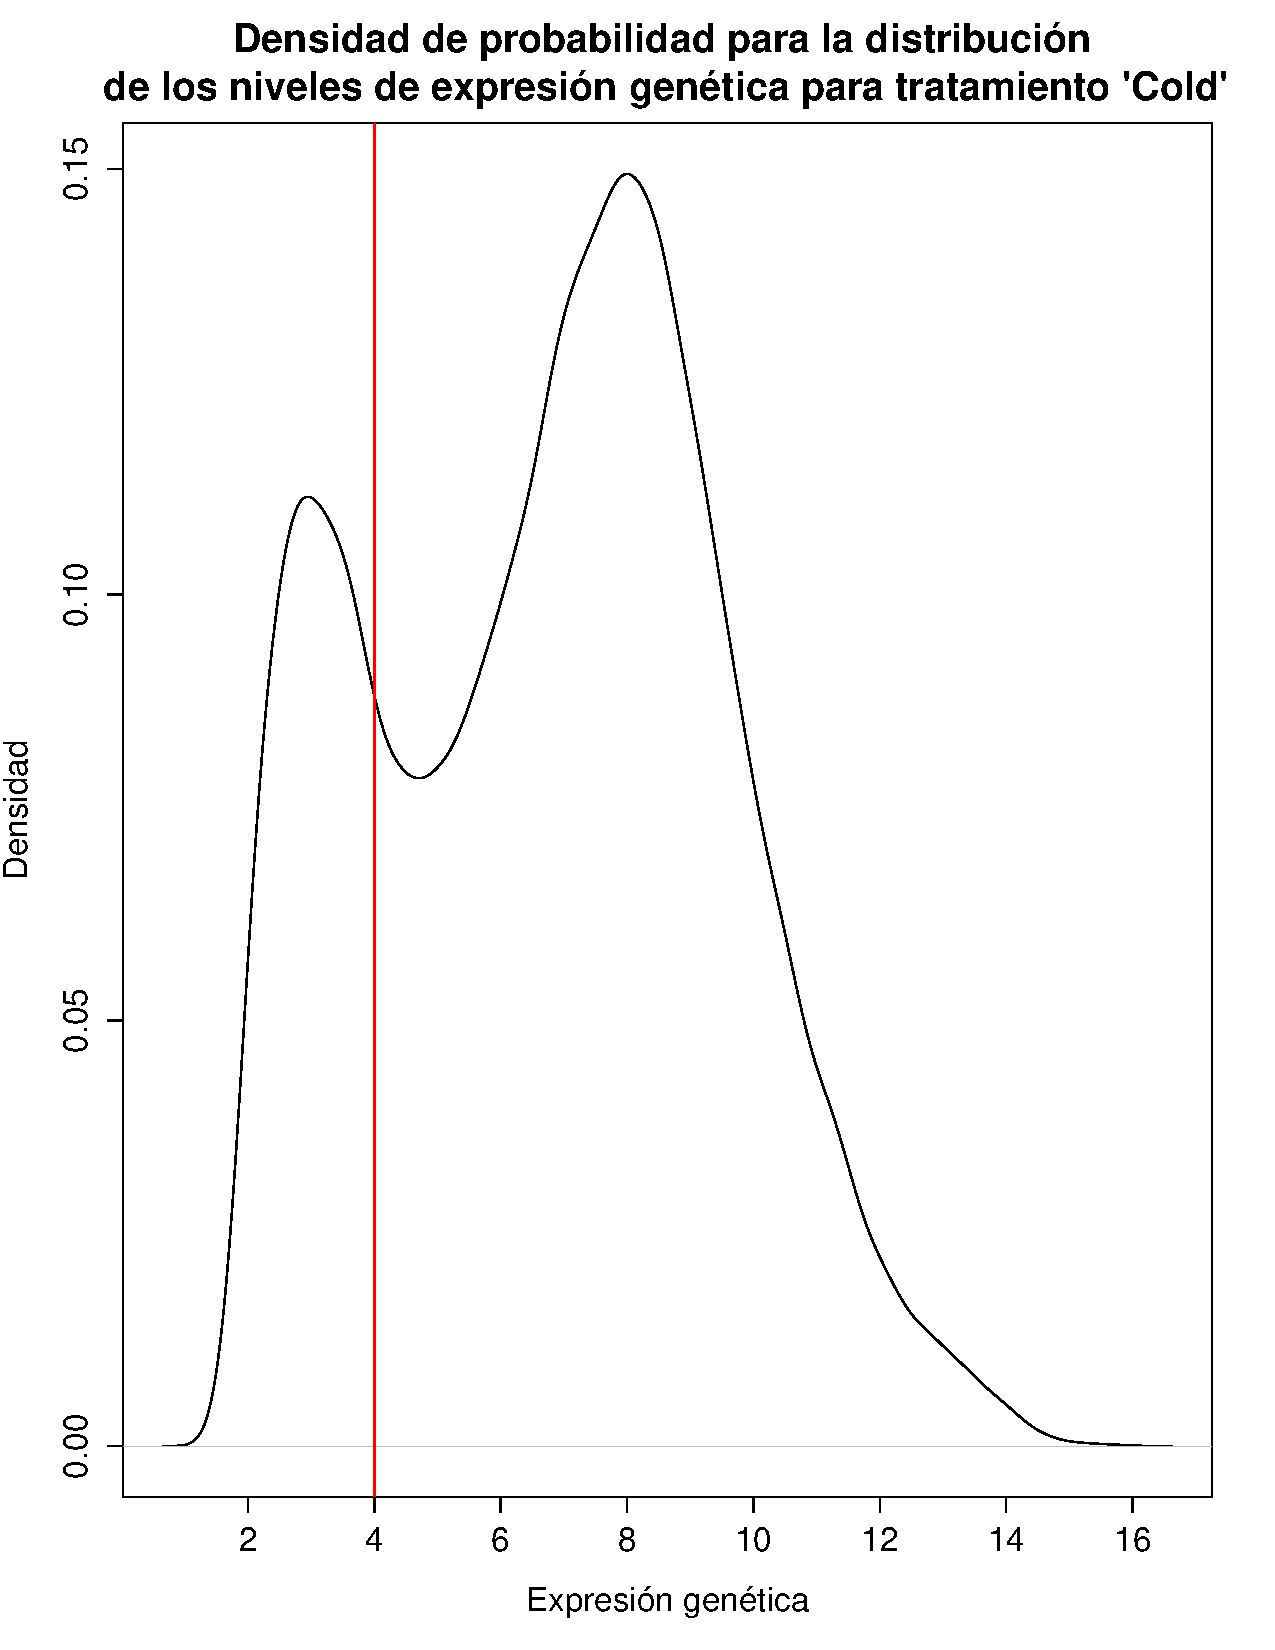
\includegraphics[width=1\textwidth]{densidad_para_niveles.pdf}
    \caption{Distribución de probabilidad para los niveles de expresión para el tratamiento 'Frío'. Todos los genes con un nivel de expresión menor al indicado por la recta vertical roja son descartados.}
    \label{fig:densidad_para_niveles}
    \end{subfigure}
    \caption{Funciones de distribución de probabilidad para perfiles de expresión génica del tratamiento 'Frío'.}
\end{figure*}
La tabla \ref{tabla:genes_por_tratamiento} muestra los filtros aplicados y la cantidad de genes finales por tratamiento.
Una vez aplicados los filtros y obtenido los genes de mayor variabilidad en su expresión, se estandarizaron los datos obtenidos para poner a todos los genes en igualdad de condiciones y pesarlos de la misma forma en el agrupamiento. Un procedimiento normal de estandarización de genes para que cada gen tenga media cero y varianza unitaria implica realizar la transformación:
\begin{equation}
	\tilde{x_i} = \frac{x_i-\bar{x}}{s_x}
\end{equation}
Con $x_i$ cada observación del gen $x$ a lo largo del tiempo para un determinado tratamiento. Una vez realizado el filtrado y estandarizado procedimos a agrupar los datos mediante los diferentes métodos mencionados en el capítulo 3.
\begin{table}[t]
  \centering
\begin{tabular}{| l | c | c | c |}
\hline
Tratamiento & $\sigma$ & A & Cantidad de genes \\
\hline
Control & 0.37 & 4 & 1885 \\
\hline
Frío & 0.71 & 3 & 1955 \\
\hline
Osmótico & 0.71 & 3 & 1923 \\
\hline
Sal & 0.88 & 3 & 1927 \\
\hline
Sequía & 0.54 & 4 & 1870 \\
\hline
Genotóxico & 0.46 & 3 & 1899 \\
\hline
Oxidativo & 0.41 & 3 & 1880 \\
\hline
UV-B & 0.51 & 4 & 1872 \\
\hline
Heridas & 0.41 & 4 & 1877 \\
\hline
Calor & 0.75 & 2 & 1960 \\
\hline
Calor y recuperación & 0.65 & 2 & 1944 \\
\hline                                         
\end{tabular}
\caption{Filtros utilizados por tratamiento y cantidad de genes luego del filtrado.}
\label{tabla:genes_por_tratamiento}
\end{table}
\section{Agrupamiento con k-means}
El método de agrupamiento k-means hace uso de la distancia euclidiana para minimizar la suma de los cuadrados. Si los datos están estandarizados y centrados, es posible relacionar la distancia euclidiana $d$ con el coeficiente de correlación mediante la fórmula:
\begin{equation}
	d(\vec{x}, \vec{y}) = \sqrt{2(n-1)(1-r(\vec{x}, \vec{y}))}
\end{equation}
con $n$ la dimensión del espacio y por lo tanto, para datos estandarizados, la distancia euclidiana se comportará de forma similar a la distancia de correlación y podremos utilizar el método k-means.\\\\
Para decidir el k a utilizar en el método, se realizó un barrido variando k entre $k=2$ y $k=30$ con pasos de 1. Al tratarse de un método heurístico, no existe garantía de convergencia al óptimo global y el resultado del mismo puede entonces depender de los grupos iniciales. Por lo tanto, para cada k, se realizaron mil agrupamientos y se midieron los índices de validación internos Calinski-Harabasz y Dunn en cada uno, definidos respectivamente como:
\begin{equation}
	CH_k = \frac{SS_B}{SS_W}\frac{n-k}{n-1}
\end{equation}
con $SS_B$ el promedio de la varianza entre grupos, $SS_W$ el promedio de la varianza intra grupos, k el número de grupos y n el número de observaciones y:
\begin{equation}
	DI = \frac{min\delta}{\max\Delta}
\end{equation}
con $\delta$ la menor de las de distancias entre grupos y $\Delta$ la mayor de las distancias intra grupos.\\\\
Grupos bien definidos tendrán distancias grandes entre ellos comparados con las distancias intra grupos, por lo que a mayor $CH$ o $DI$, mejor definidos estarán los grupos.\\\\
Las figuras \ref{fig:barrido_k_ch} y \ref{fig:barrido_k_dunn} muestran un gráfico de caja (o boxplot en inglés), para el índice CH y Dunn respectivamente para cada uno de los k en el barrido. Un boxplot consiste en una caja con una linea horizontal que indica el segundo cuartil, es decir, la mediana del conjunto de datos, y dos lineas verticales llamadas bigotes (o whiskers en inglés) que se extiende una desde el primer cuartil hasta el valor más pequeño del conjunto (con excepción de puntos aislados) y la otra desde el tercer cuartil hasta el valor más grande. Los puntos aislados se grafican de forma separada en el gráfico.
\clearpage
\begin{figure*}[t!]
    \centering
    \begin{subfigure}[t]{0.7\textwidth}
    \centering
    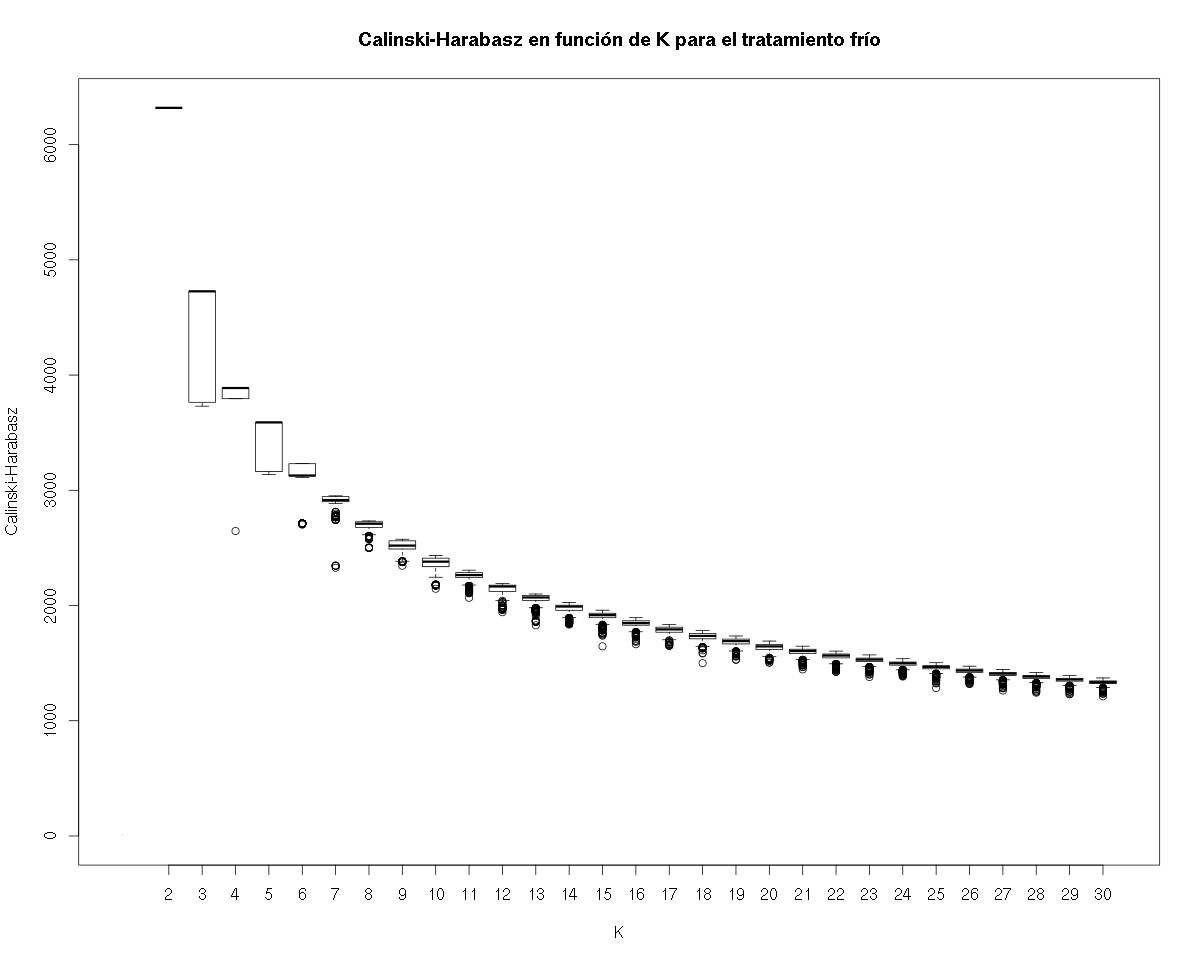
\includegraphics[width=1\textwidth]{barrido_k_ch}
    \caption{Índice CH de particiones realizadas con k-means para k entre 2 y 30.}
    \label{fig:barrido_k_ch}
    \end{subfigure}
    \begin{subfigure}[t]{0.7\textwidth}
    \centering
    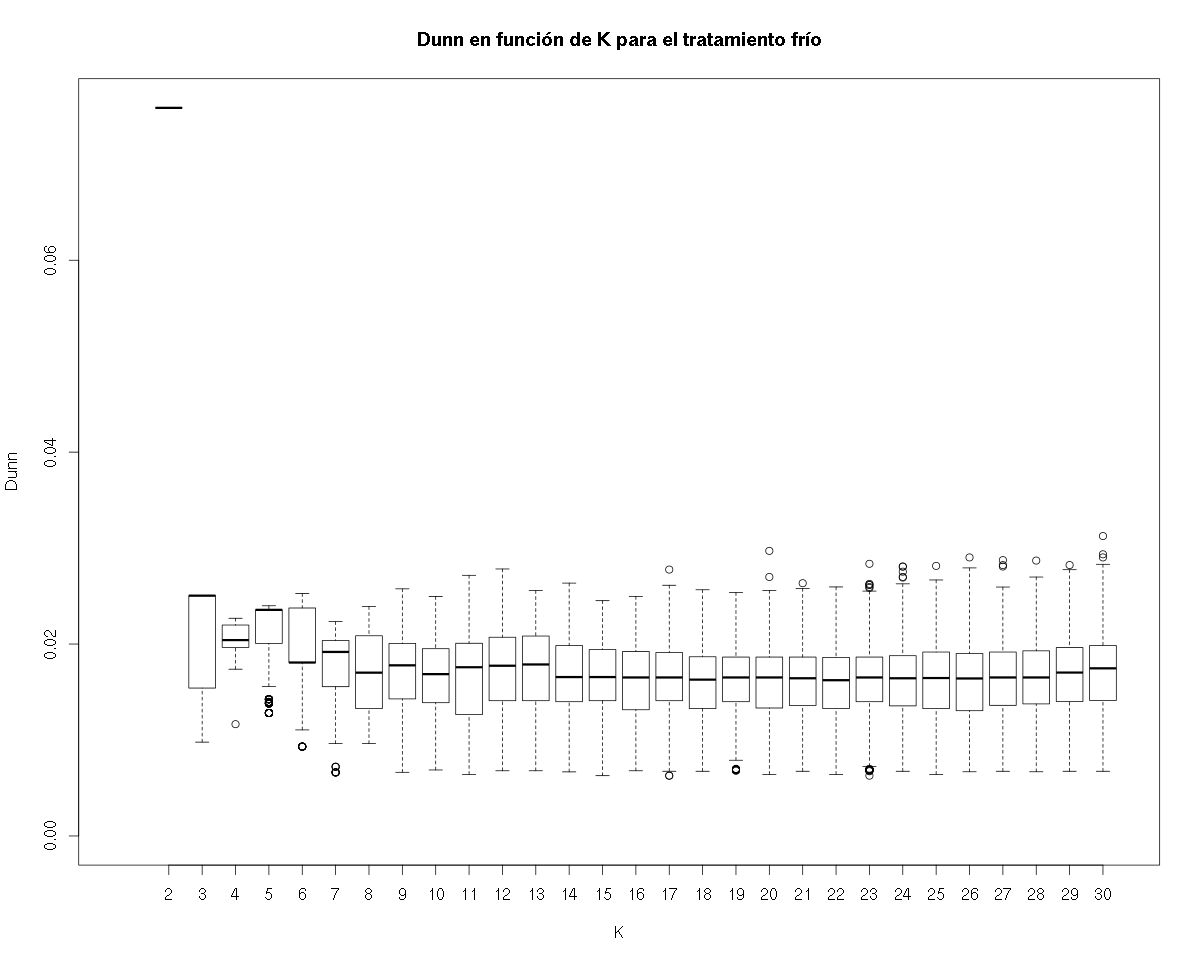
\includegraphics[width=1\textwidth]{barrido_k_dunn}
    \caption{Índice Dunn de particiones realizadas con k-means para k entre 2 y 30.}
    \label{fig:barrido_k_dunn}
    \end{subfigure}
    \caption{Índices de validación interna para particiones realizadas con k-means}
\end{figure*}
Se observa que la cantidad de grupos que maximiza estos índices es 2. Se realizó entonces un agrupamiento con $k=2$, obteniéndose los perfiles que muestra la figura \ref{fig:perfiles_k_means}, con una correlación media de $\rho=0.74$ para el primero y de  $\rho=0.79$ para el segundo, con aproximadamente el 50\% de los genes en cada grupo.
\begin{figure}[h]
    \centering
    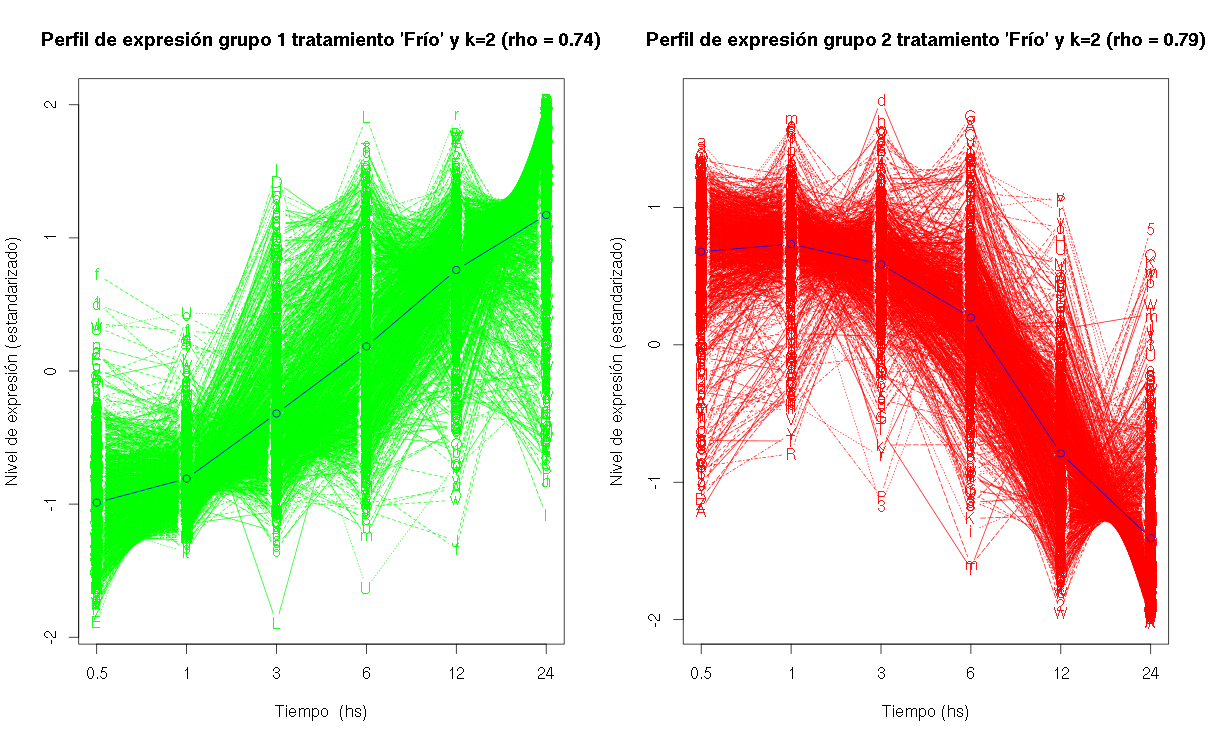
\includegraphics[width=1\textwidth]{perfiles_k_means}
    \caption{Perfiles de expresión génica obtenidos con el método k-means (k=2) para el tratamiento 'Frío'. En azul, el valor medio de cada grupo.}
    \label{fig:perfiles_k_means}
\end{figure}
Estas estructuras tan grandes son de difícil interpretación biológica, ya que si bien las respuestas de expresión dentro de cada grupo son similares, existe mucha heterogeneidad en las funciones biológicas de los genes que los componen. Esto se debe a que el método k-means está trabajando a una escala que no permite extraer información biológica de los grupos. Será necesario entonces aumentar la granularidad mediante la consideración de otros métodos de agrupamiento.
\section{Agrupamiento con corte de árbol dinámico}
Utilizando el método de corte de árbol dinámico se realizó un agrupamiento para cada tratamiento, utilizando alternativamente los parámetros $deepSplit=1$ (que llamaremos $ds1$, de menor granularidad) y $deepSplit=4$ (que llamaremos $ds4$, de mayor granularidad). Las figuras \ref{ref:histograma_ds_1} y \ref{ref:histograma_ds_4} presentan histogramas de los tamaños de los grupos obtenidos, en escala logarítmica, para cada método. Se observa que $ds1$ llega a tener grupos de mayor tamaño que $ds4$ pero menor cantidad de grupos en total. Esto es esperable ya que una variación en el parámetro $deepsplit$ aumenta o disminuye la granularidad del método.\\
\begin{sidewaysfigure}[H]
    \centering
    \begin{subfigure}[t]{0.45\textwidth}
    \centering
    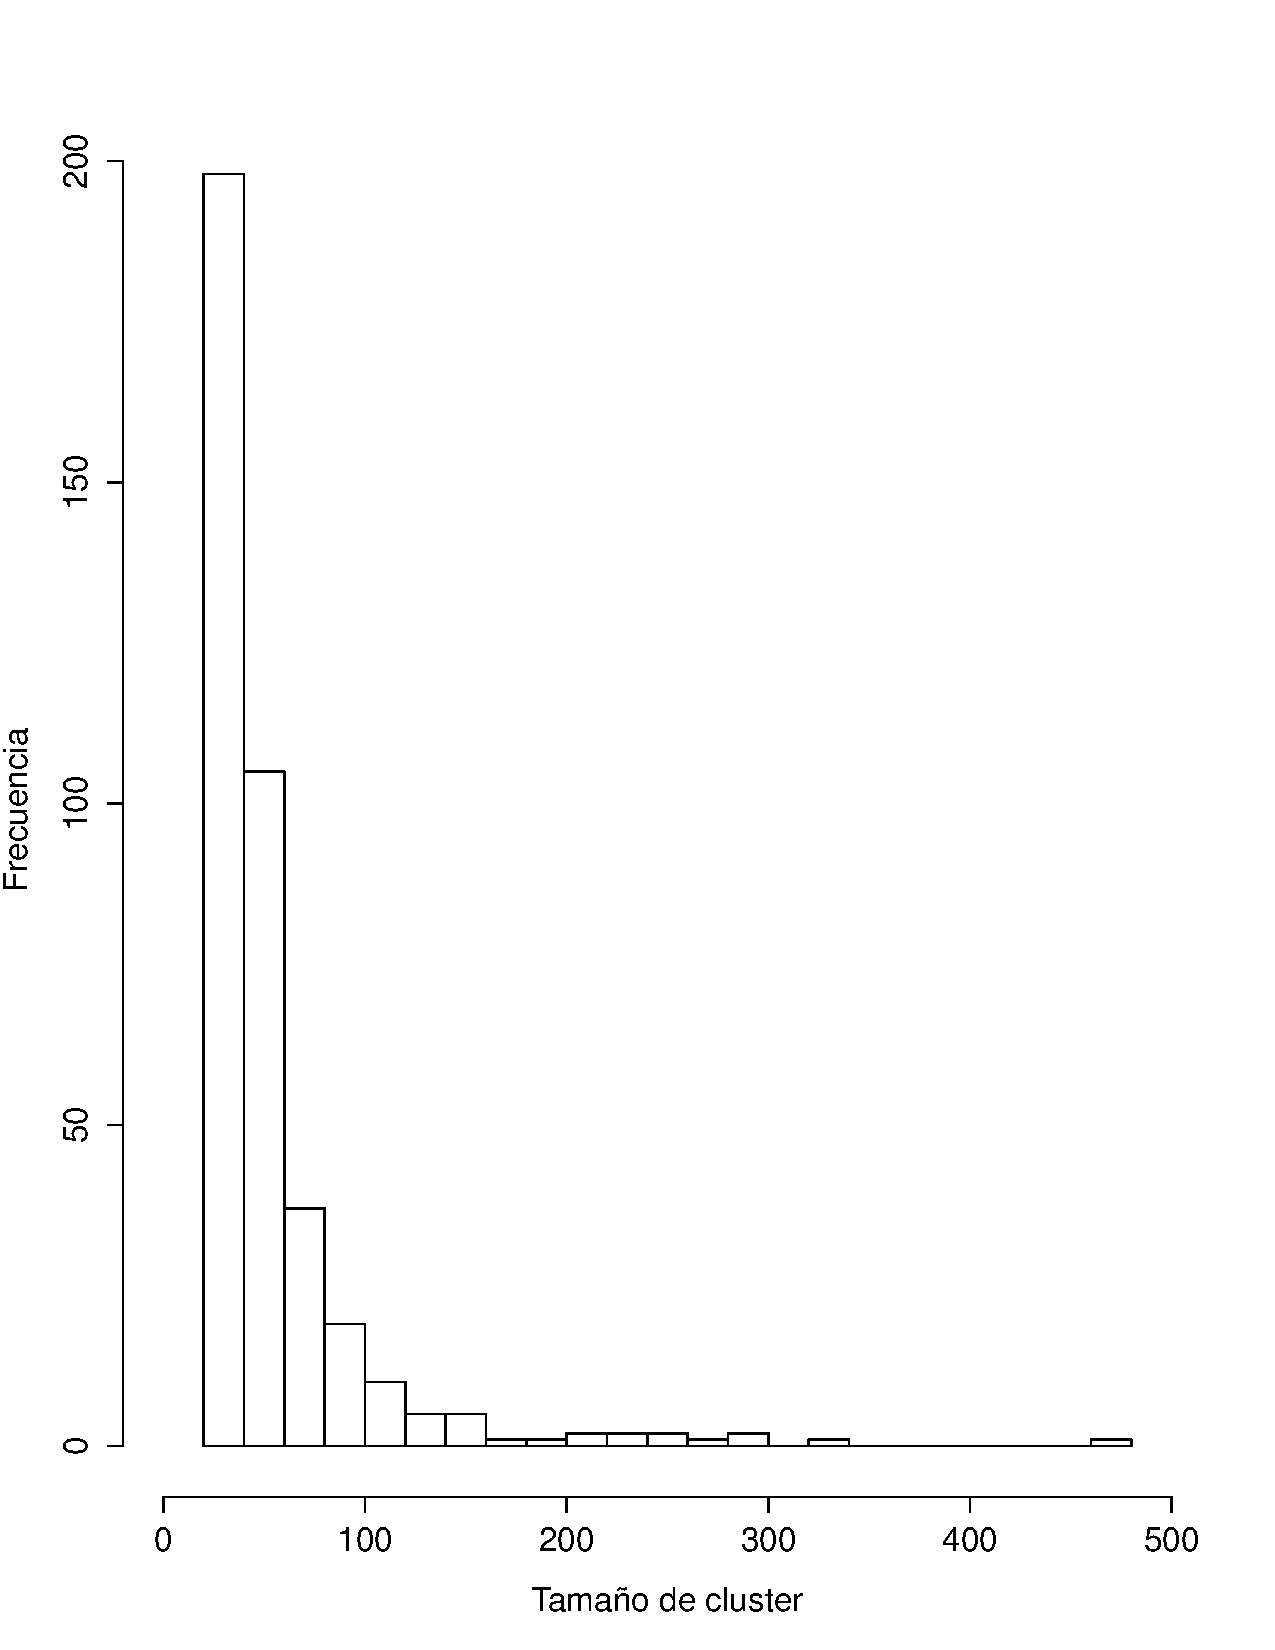
\includegraphics[width=1\textwidth]{histograma_ds_1.pdf}
    \caption{Histograma de tamaños de grupos para $ds1$.}
    \label{fig:histograma_ds_1}
    \end{subfigure}
    \begin{subfigure}[t]{0.45\textwidth}
    \centering
    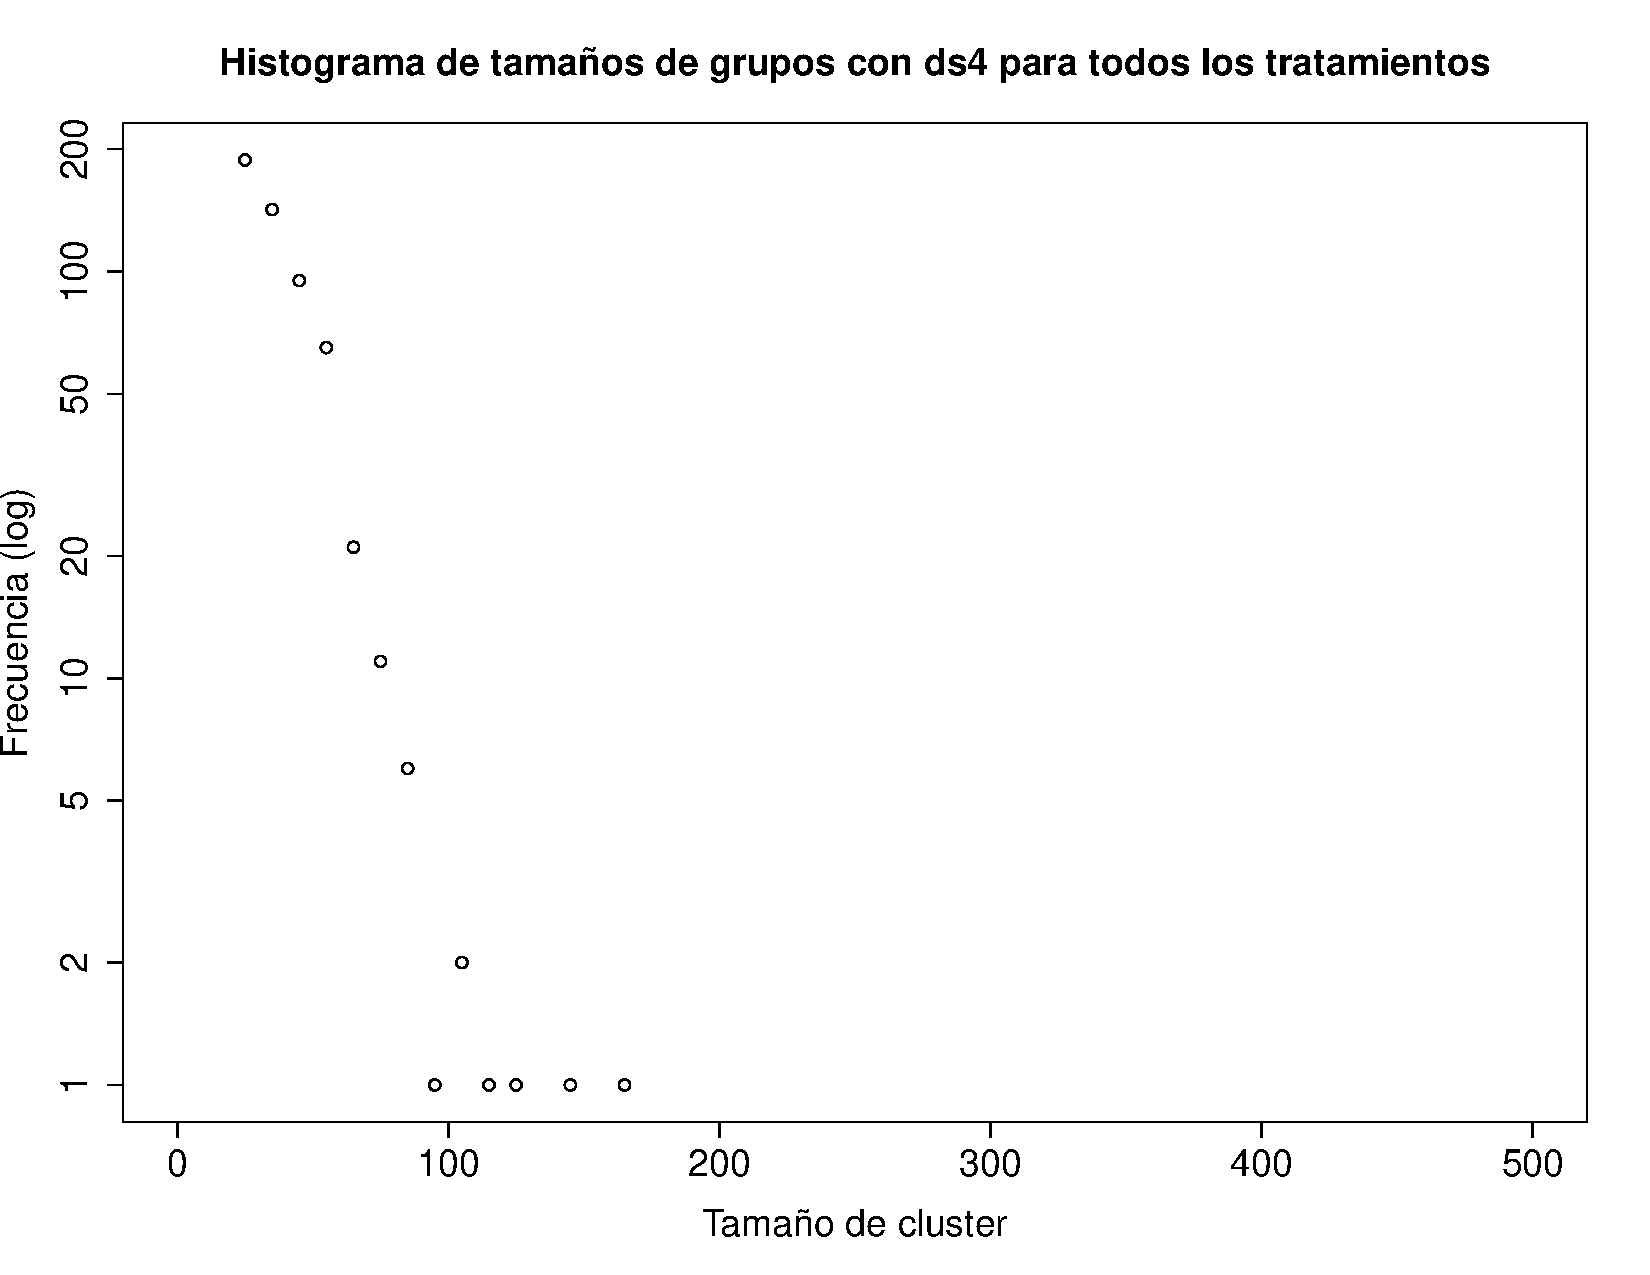
\includegraphics[width=1\textwidth]{histograma_ds_4.pdf}
    \caption{Histograma de tamaños de grupos para $ds4$.}
    \label{fig:histograma_ds_4}
    \end{subfigure}
    \caption{Histogramas de tamaños de grupos en escala logarítmica para todos los tratamientos. En el panel de la izquierda, los grupos obtenidos con $ds1$ y en el de la derecha, con $ds4$. $ds1$ presenta una mayor cantidad de grupos que $ds4$.}
\end{sidewaysfigure}
A modo ilustrativo, las figuras \ref{fig:perfiles_ds_1} y \ref{fig:perfiles_ds_4} muestran los perfiles de los 9 grupos más grandes obtenidos con cada parámetro respectivamente para el tratamiento ``Frío''.\\\\ 
En general, para todos los tratamientos, los grupos obtenidos por el método de corte de árbol dinámico tienen mayor correlación media ($\rho$) que los obtenidos por el método k-means.\\\\
\begin{sidewaysfigure}[H]
    \centering
    \begin{subfigure}[t]{0.45\textwidth}
    \centering
    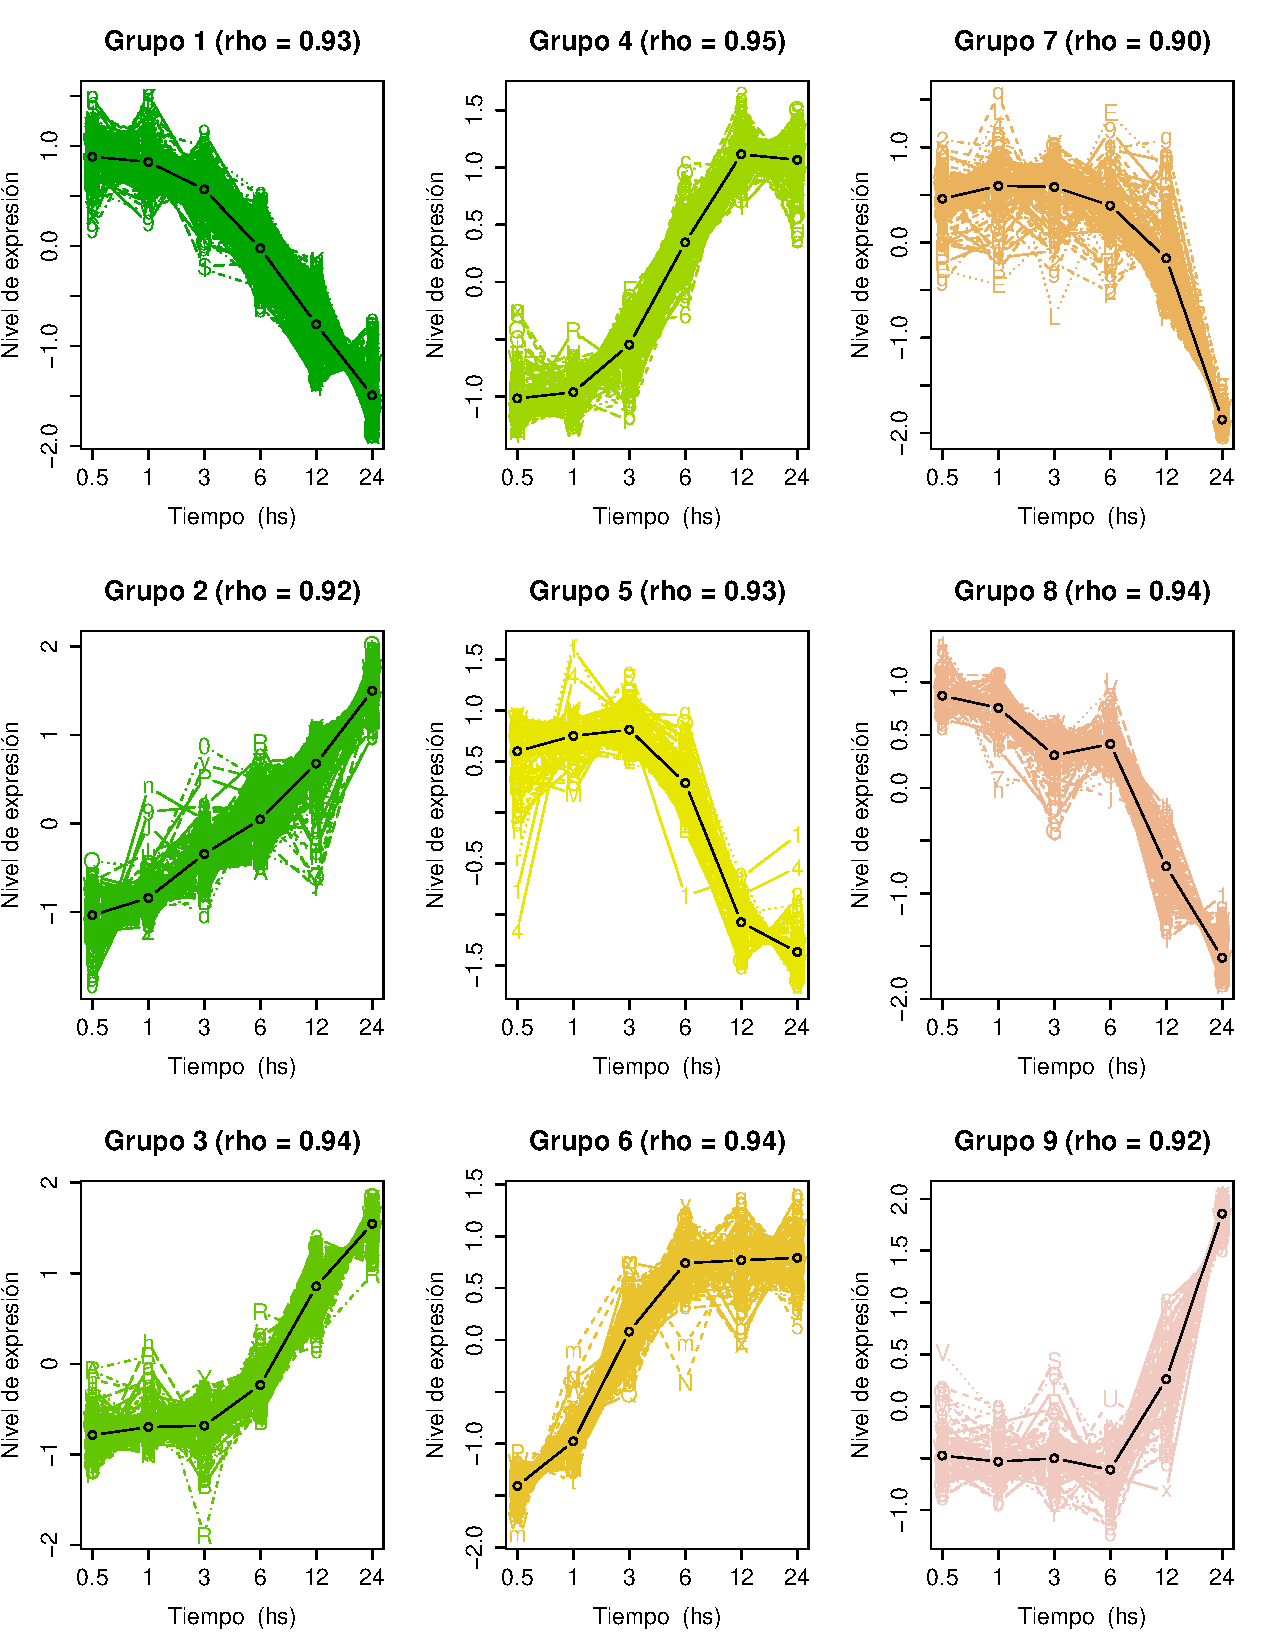
\includegraphics[width=1\textwidth]{perfiles_ds_1.pdf}
    \caption{Perfiles obtenidos con $ds1$.}
    \label{fig:perfiles_ds_1}
    \end{subfigure}
    \begin{subfigure}[t]{0.45\textwidth}
    \centering
    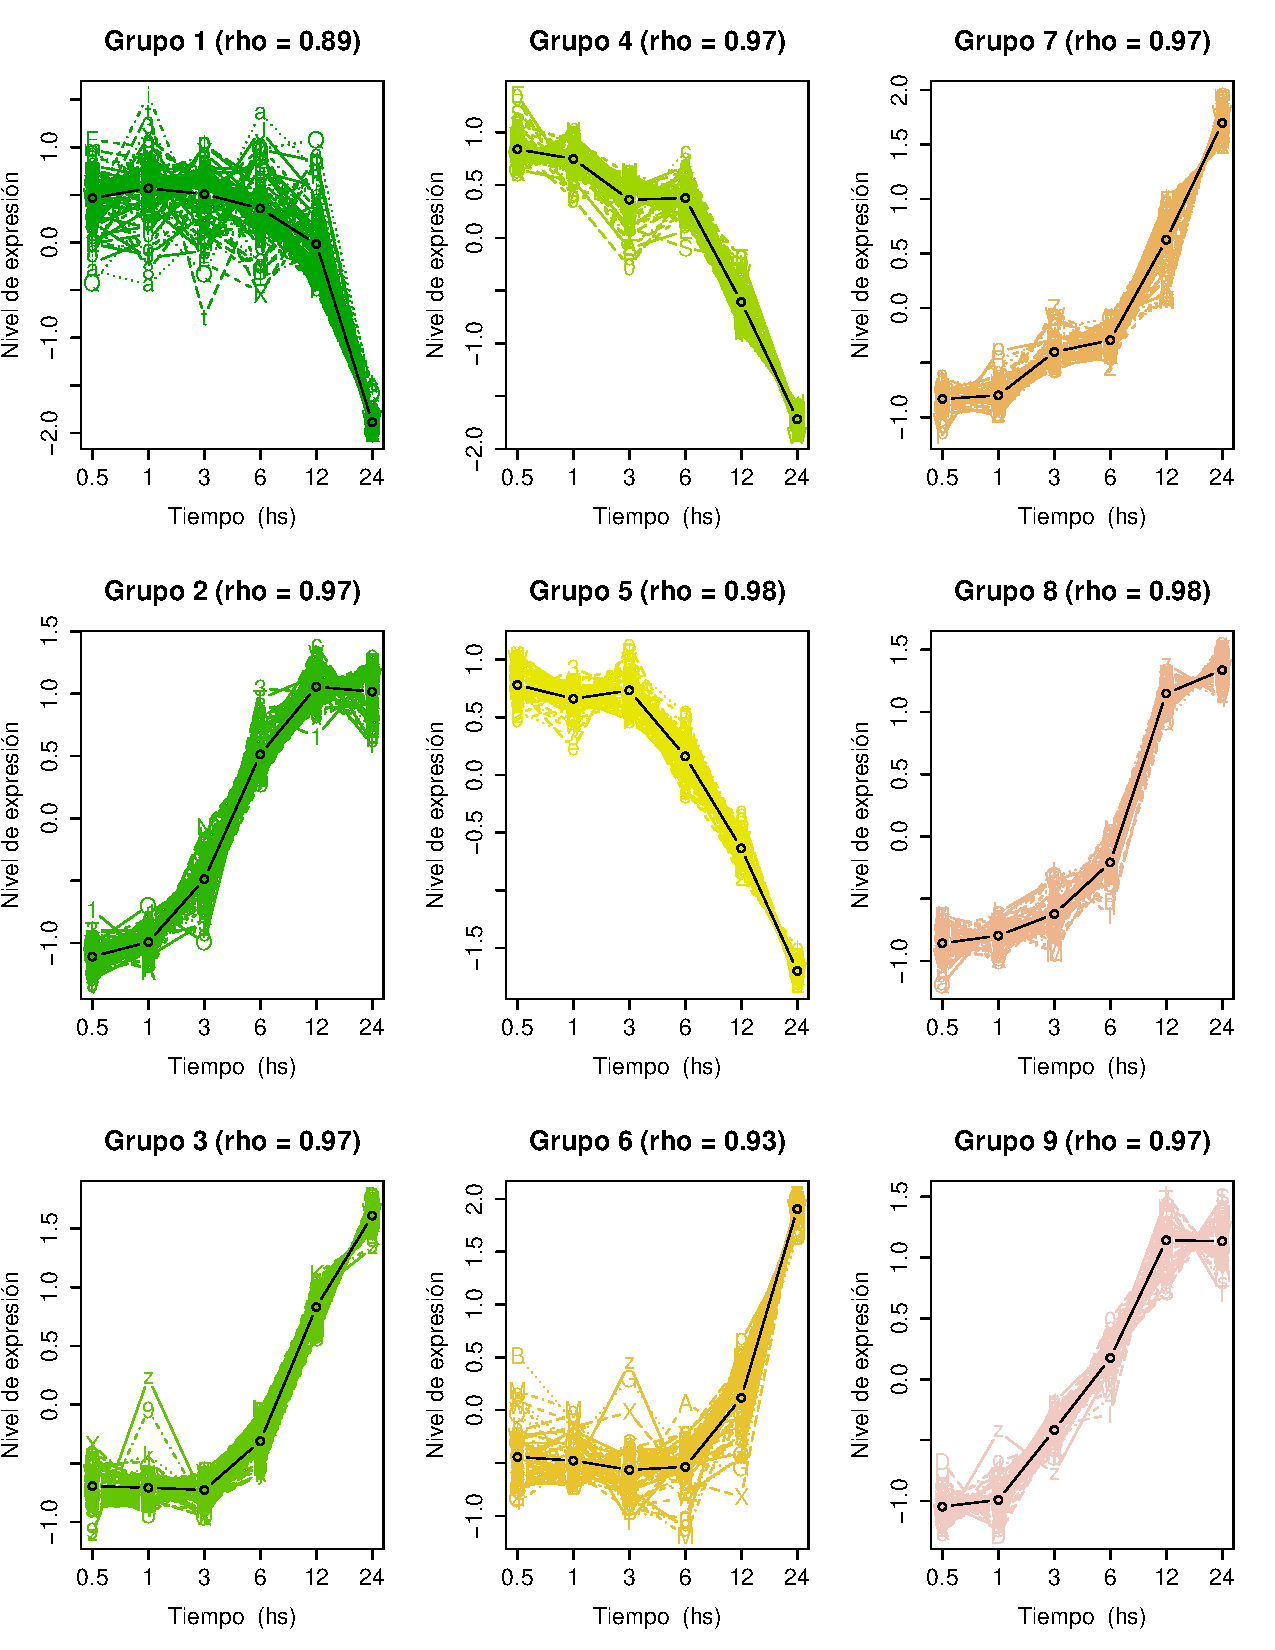
\includegraphics[width=1\textwidth]{perfiles_ds_4.pdf}
    \caption{Perfiles obtenidos con $ds4$.}
    \label{fig:perfiles_ds_4}
    \end{subfigure}
    \caption{Perfiles de expresión génica de los 9 grupos más grandes obtenidos con el método corte de árbol dinámico para $ds1$ y $ds4$ para el tratamiento 'Frío'. En negro, el valor medio de cada grupo. En el título se consigna la correlación media de cada uno (rho).}
\end{sidewaysfigure}
Para cada parámetro, cada tratamiento y cada grupo, se realizó un control nulo consistente en tomar la misma cantidad de genes presentes en el grupo, pero de forma aleatoria, del conjunto de genes que formaban el tratamiento, y medir su correlación media. Esto se realizó 1000 veces para cada grupo. Las figuras \ref{ref:correlacion_media_por_tamano_ds_1} y \ref{ref:correlacion_media_por_tamano_ds_4} muestran la correlación media por tamaño de grupo y el control nulo para $ds1$ y $ds4$ respectivamente. Los grupos fueron agrupados por tamaño de a 10 genes, donde los colores más claros indican mayor cantidad de grupos que los oscuros. El gráfico tiene además la media, en negro, y el segundo y tercer cuartil, en gris, para la distribución del control nulo.
\begin{sidewaysfigure}[H]
    \centering
    \begin{subfigure}[t]{0.45\textwidth}
    \centering
    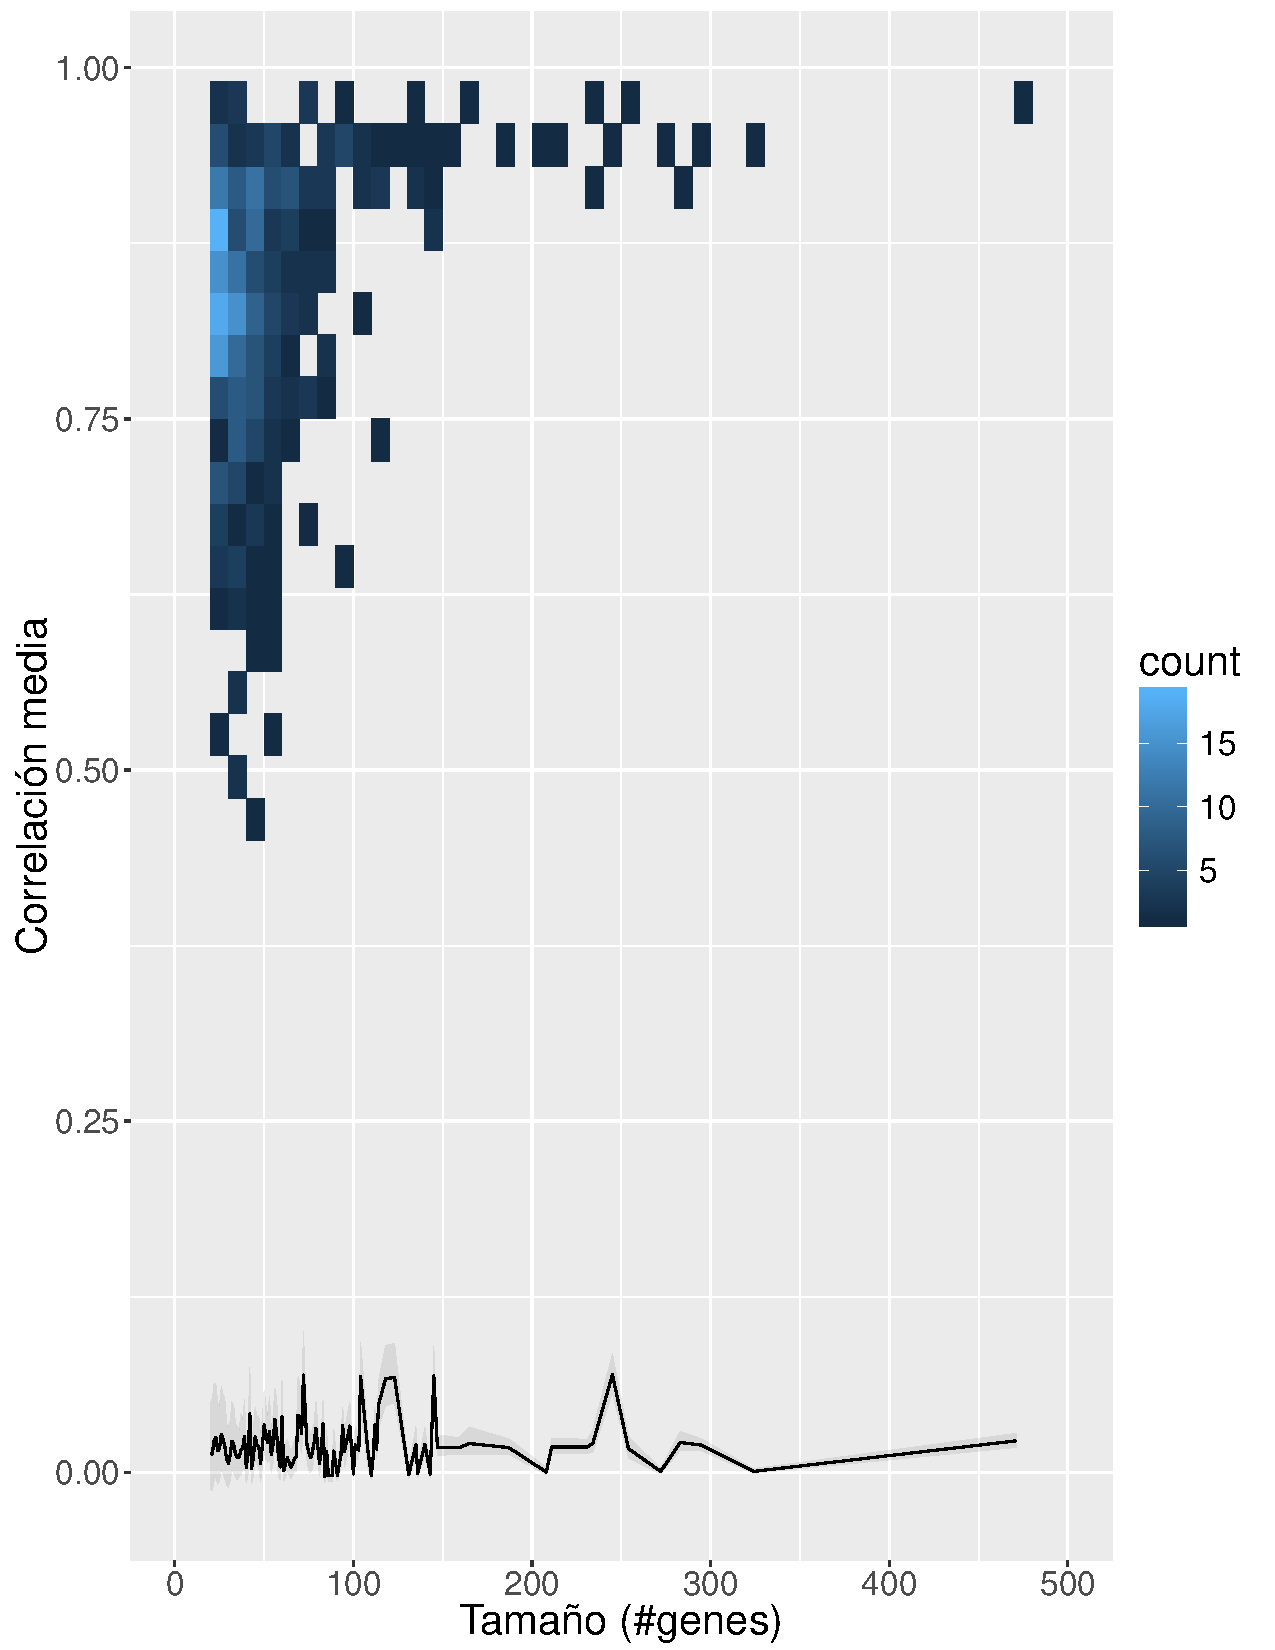
\includegraphics[width=1\textwidth]{correlacion_media_por_tamano_ds_1.pdf}
    \caption{Correlación media por tamaño de grupo para $ds4$.}
    \label{fig:correlacion_media_por_tamano_ds_1}
    \end{subfigure}
    \begin{subfigure}[t]{0.45\textwidth}
    \centering
    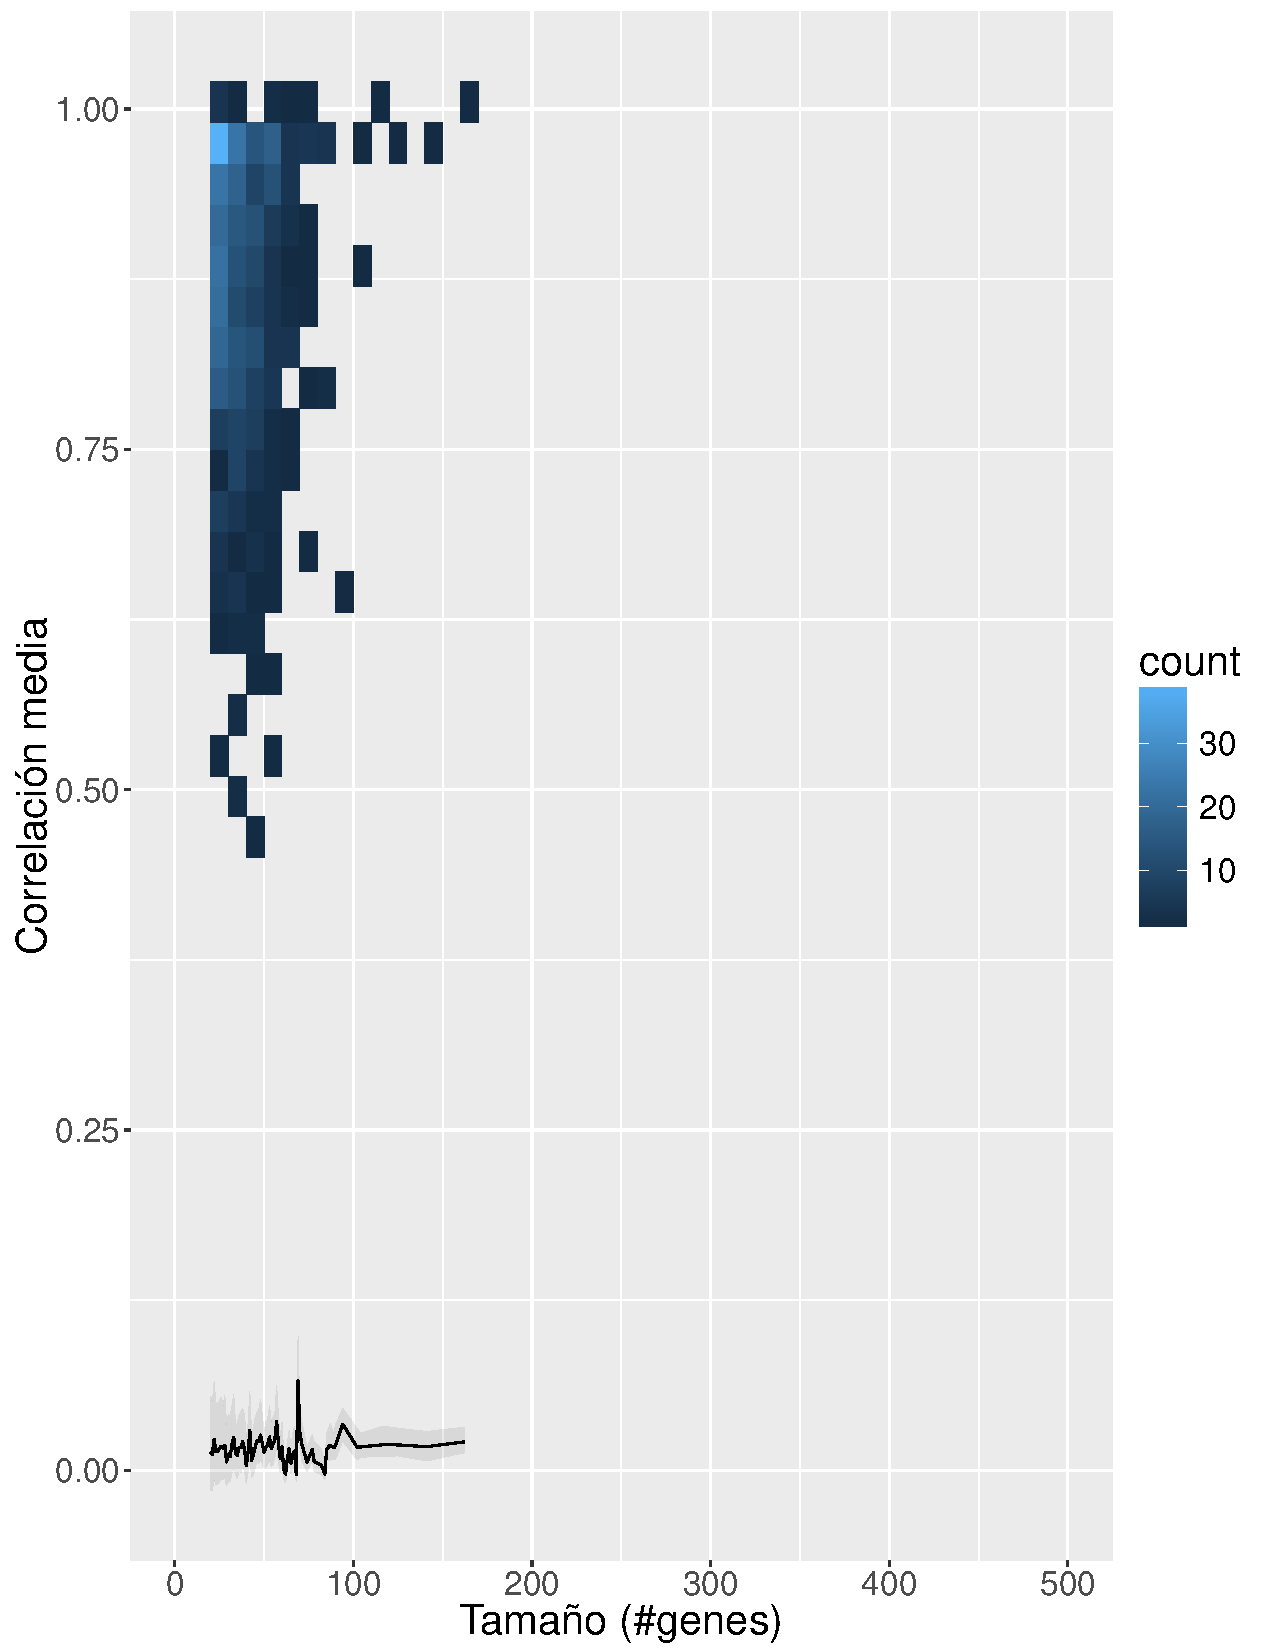
\includegraphics[width=1\textwidth]{correlacion_media_por_tamano_ds_4.pdf}
    \caption{Correlación media por tamaño de grupo para $ds4$.}
    \label{fig:correlacion_media_por_tamano_ds_4}
    \end{subfigure}
    \caption{Correlación media por tamaño de grupo para los grupos obtenidos por corte de árbol dinámico con $ds1$, $ds4$ y control nulo para todos los tratamientos en mapa de colores o heatmap. Los grupos fueron agrupados por tamaño de a 10 genes, donde los colores más claros indican mayor cantidad de grupos que los oscuros. Se consigna la media, en negro, y el segundo y tercer cuartil, en gris, para la distribución del control nulo.}
\end{sidewaysfigure}
Se observa que la correlación media de los grupos es en todos los casos notoriamente superior a la del control nulo. Esto muestra que existe estructura no trivial en los grupos hallados para ambos parámetros. \\\\
Estos grupos de $ds1$ comparativamente grandes tienen alta correlación. Sin embargo hay una menor correlación en los grupos pequeños para $ds1$ que para $ds4$. Una posible explicación para esto es que para que exista un grupo grande, es necesario que el mismo tenga alta correlación. De lo contrario, el método buscará partirlo en grupos más chicos hasta maximizar la correlación de cada grupo.\\\\
\clearpage
\section{Comparación de escalas de resolución de los métodos}
Otra forma de visualizar la diferencia en los tamaños de los grupos que obtiene cada método es mediante la función de distribución acumulada empírica que se observa en la figura \ref{fig:ecdf_k_ds1_ds4}. En la misma se observa que corte de árbol dinámico con $ds4$ produce la mayor cantidad de grupos con los menores tamaños, seguida por la misma técnica pero con $ds1$ y finalmente por k-means con solamente dos grupos muy masivos.
\begin{figure}[h]
    \centering
    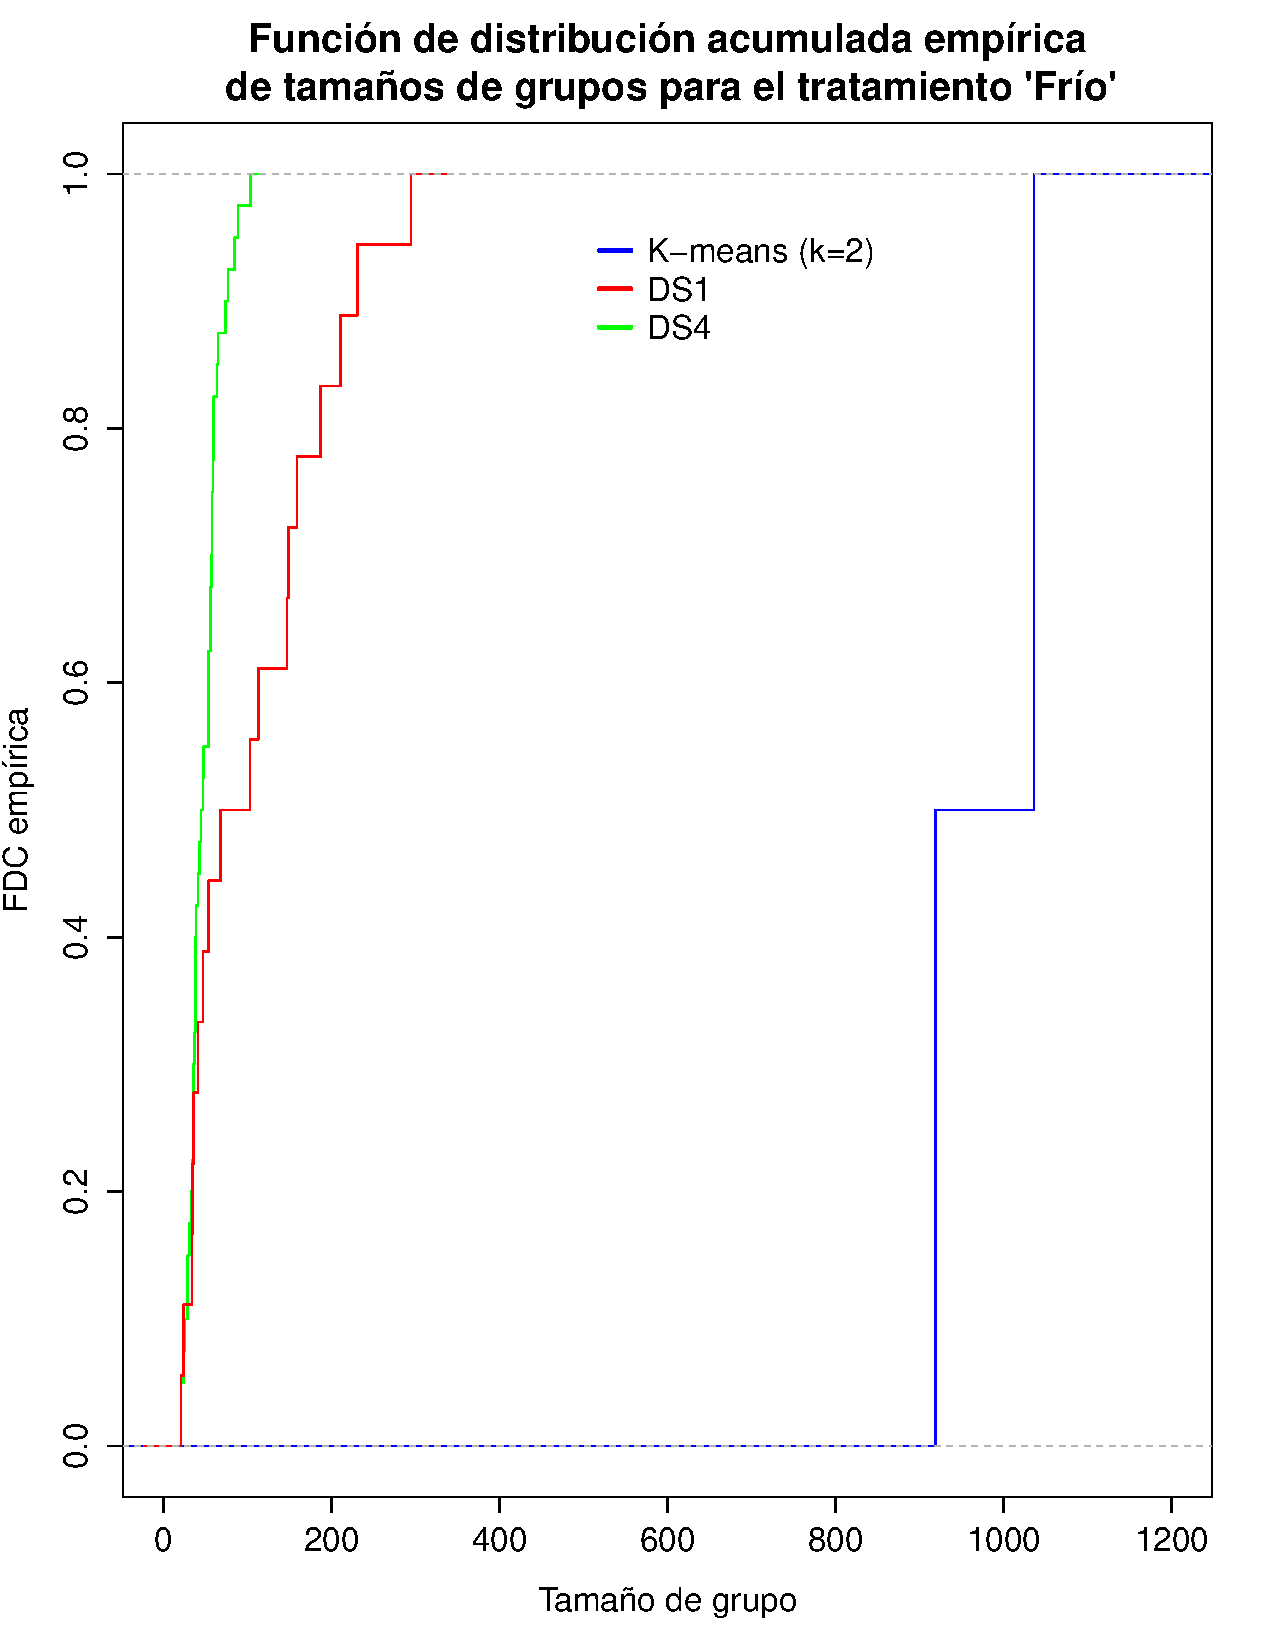
\includegraphics[width=0.9\textwidth]{ecdf_k_ds1_ds4.pdf}
    \caption{Función de distribución acumulada empírica en función del tamaño de grupo para los métodos k-means (k=2) en azul, $ds1$ en rojo y $ds4$ en verde para el tratamiento 'Frío'.}
    \label{fig:ecdf_k_ds1_ds4}
\end{figure}
Por otro lado, para poder caracterizar la granularidad de las particiones halladas con cada método, podemos calcular la fracción de los grupos más grandes de una partición en otra partición. La figura \ref{fig:fraccion_de_km_en_ds1_en_ds4} muestra como están distribuidos los dos grupos de la partición k-means en los grupos de la partición corte de árbol dinámico con $ds1$ y los 4 grupos más grandes de la partición corte de árbol dinámico con $ds1$ en la de $ds4$.
\begin{sidewaysfigure}
    \centering
    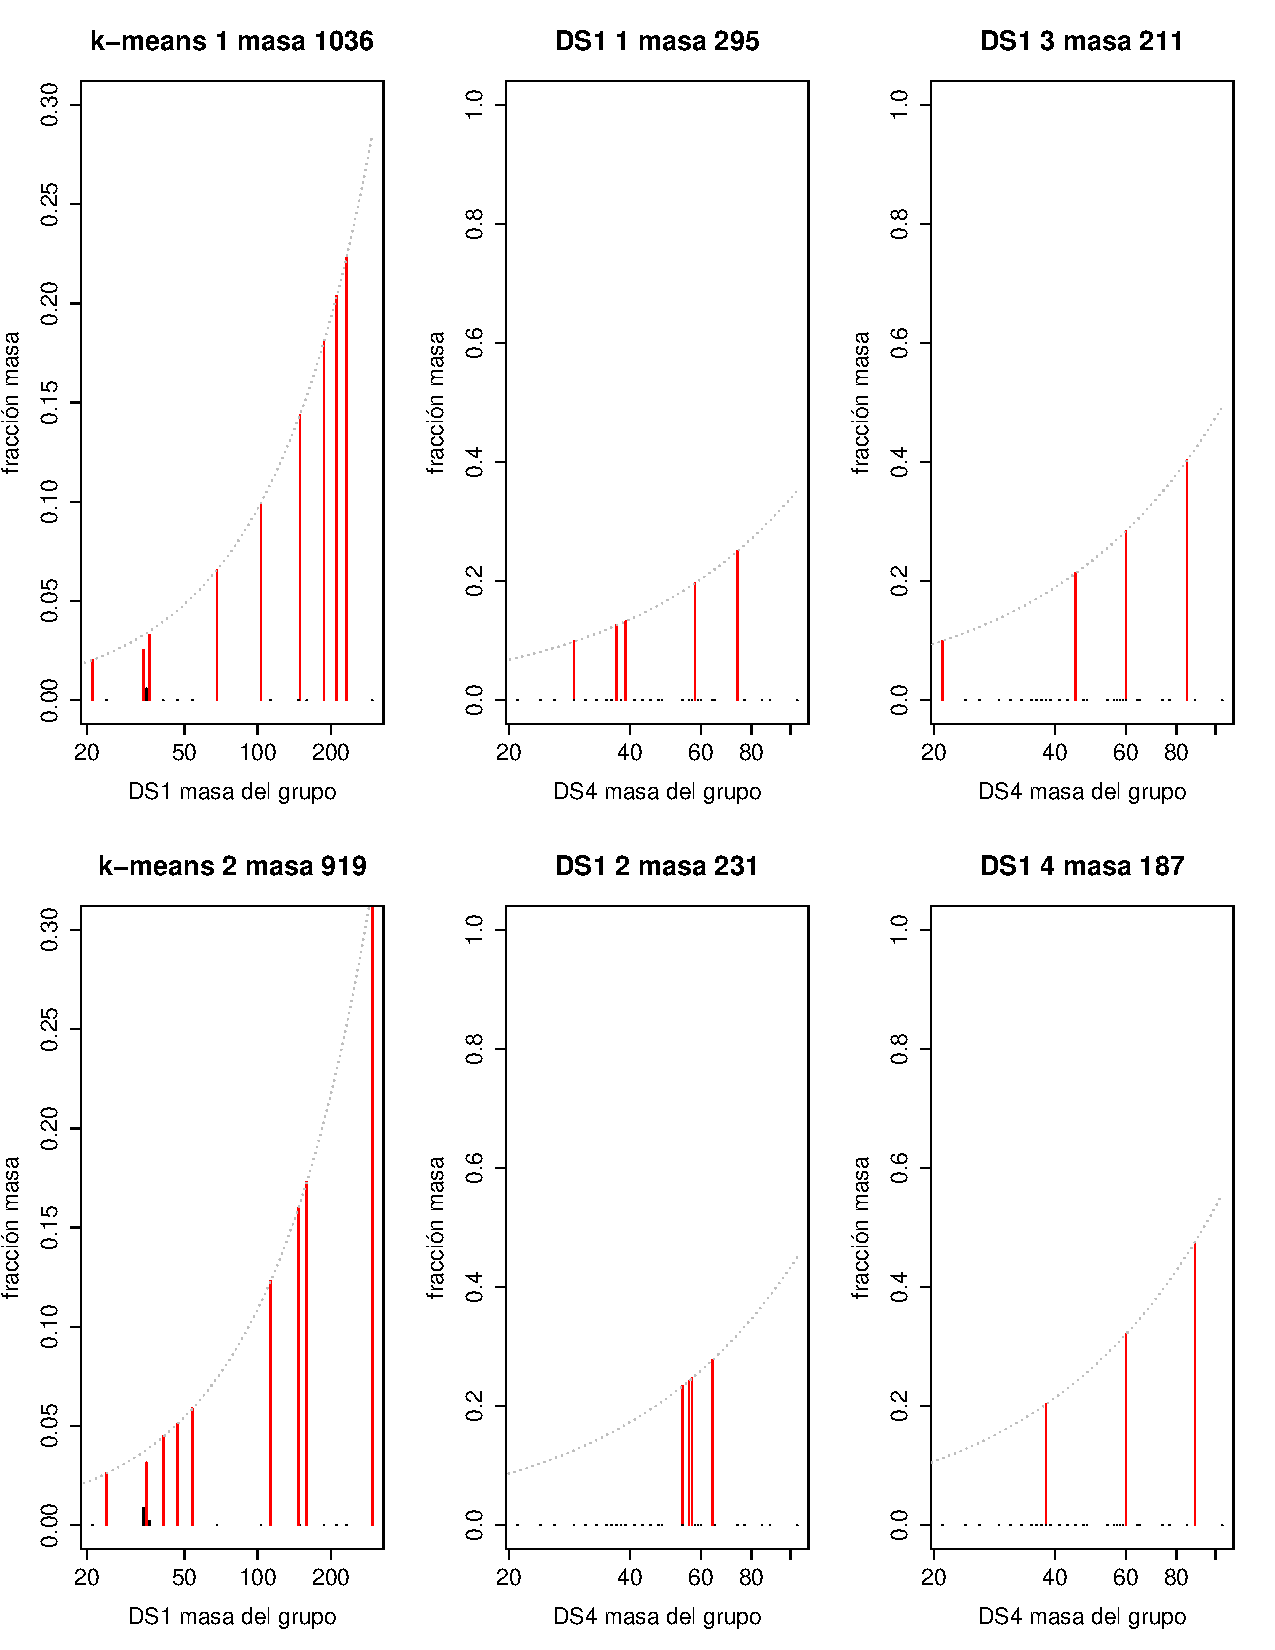
\includegraphics[width=0.6\textwidth]{fraccion_de_km_en_ds1_en_ds4.pdf}
    \caption{Fracción de grupos de una partición más fina dentro de grupos en una partición más gruesa para el tratamiento 'Frío', con $ds1$, $ds4$ y k-means. En rojo, aquellos subgrupos que están contenidos en más de un 50\% en el grupo. La linea punteada marca el porcentaje del grupo que representa el total del subgrupo.}
    \label{fig:fraccion_de_km_en_ds1_en_ds4}
\end{sidewaysfigure}
%\begin{figure*}[t!]
    %\centering
    %\begin{subfigure}[t]{0.35\textheight}
    %\centering
    %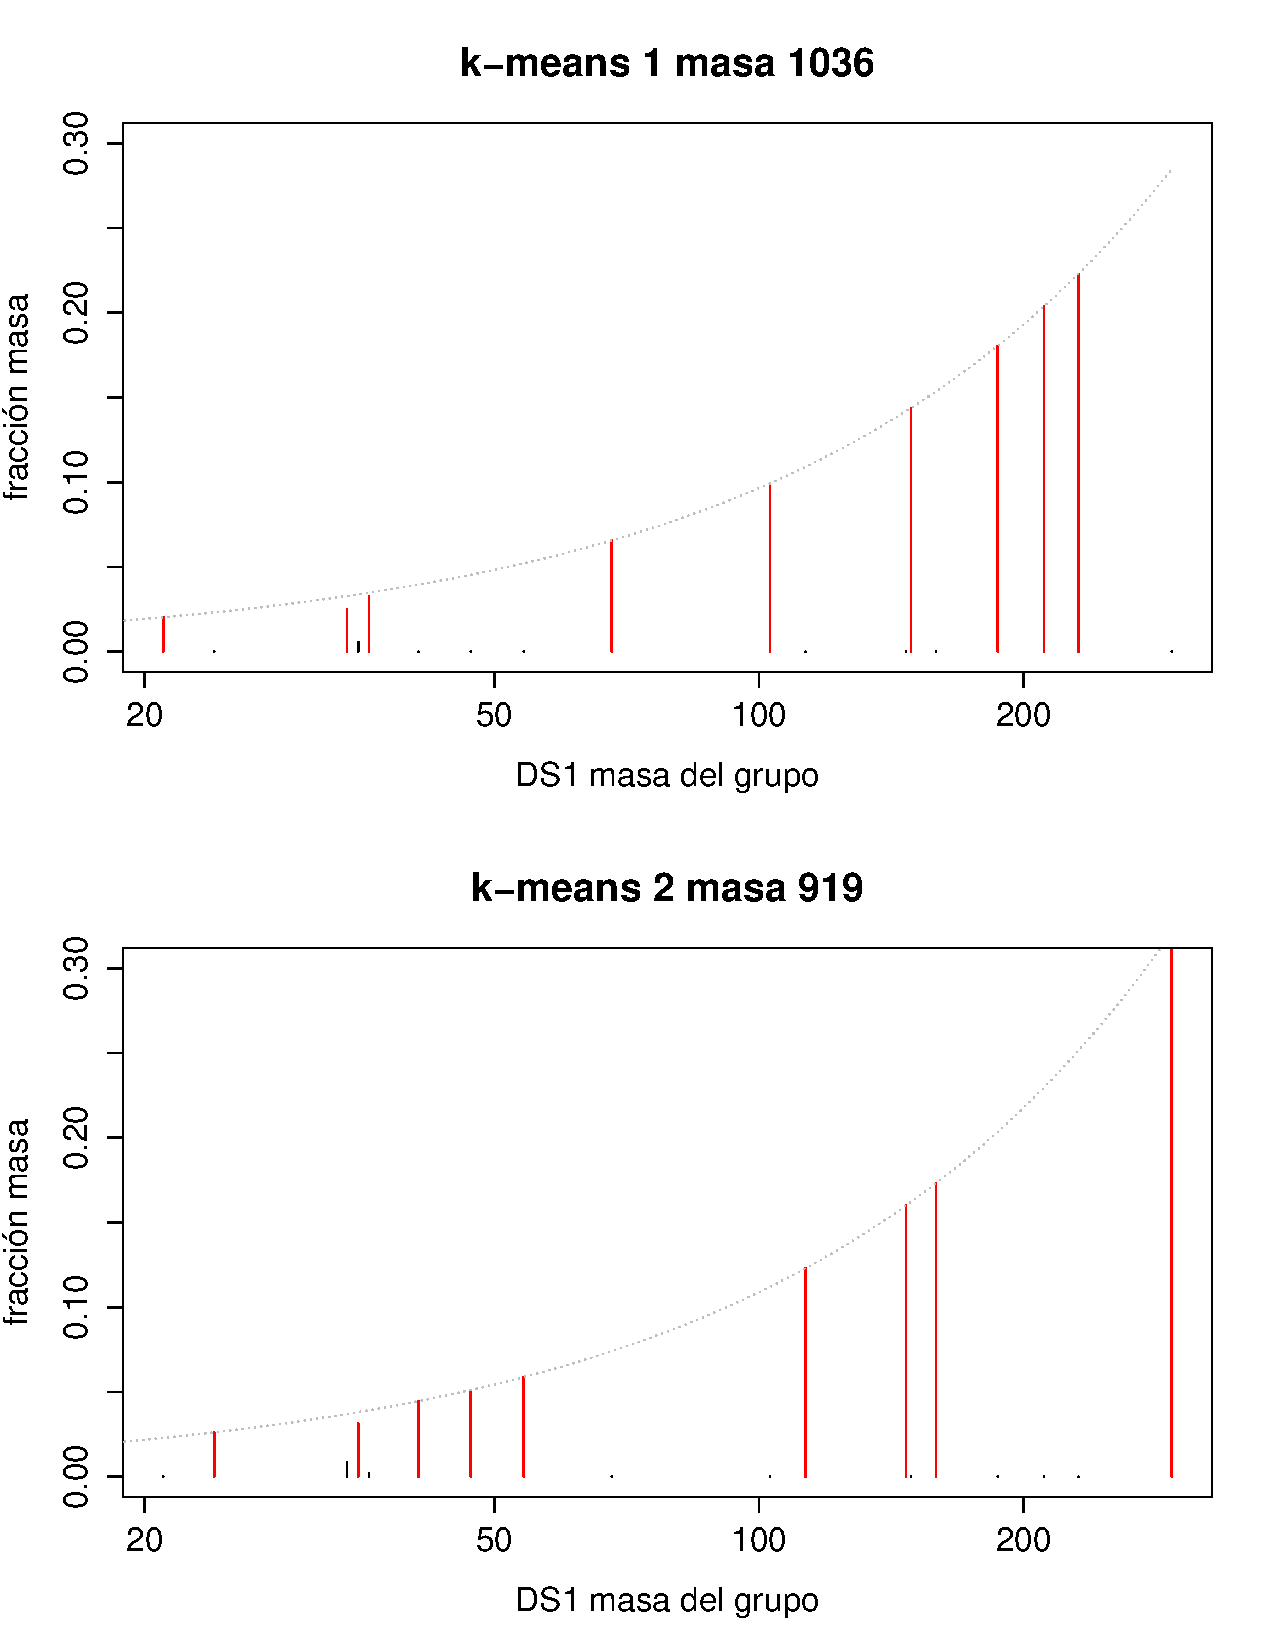
\includegraphics[width=1\textwidth]{fraccion_de_km_en_ds1.pdf}
    %\caption{Fracción de grupos de $ds1$ en los grupos k-means.}
  %%  \label{fig:fraccion_de_km_en_ds1}
 %   \end{subfigure}
    
 %   \begin{subfigure}[t]{0.35\textheight}
 %   \centering
 %%   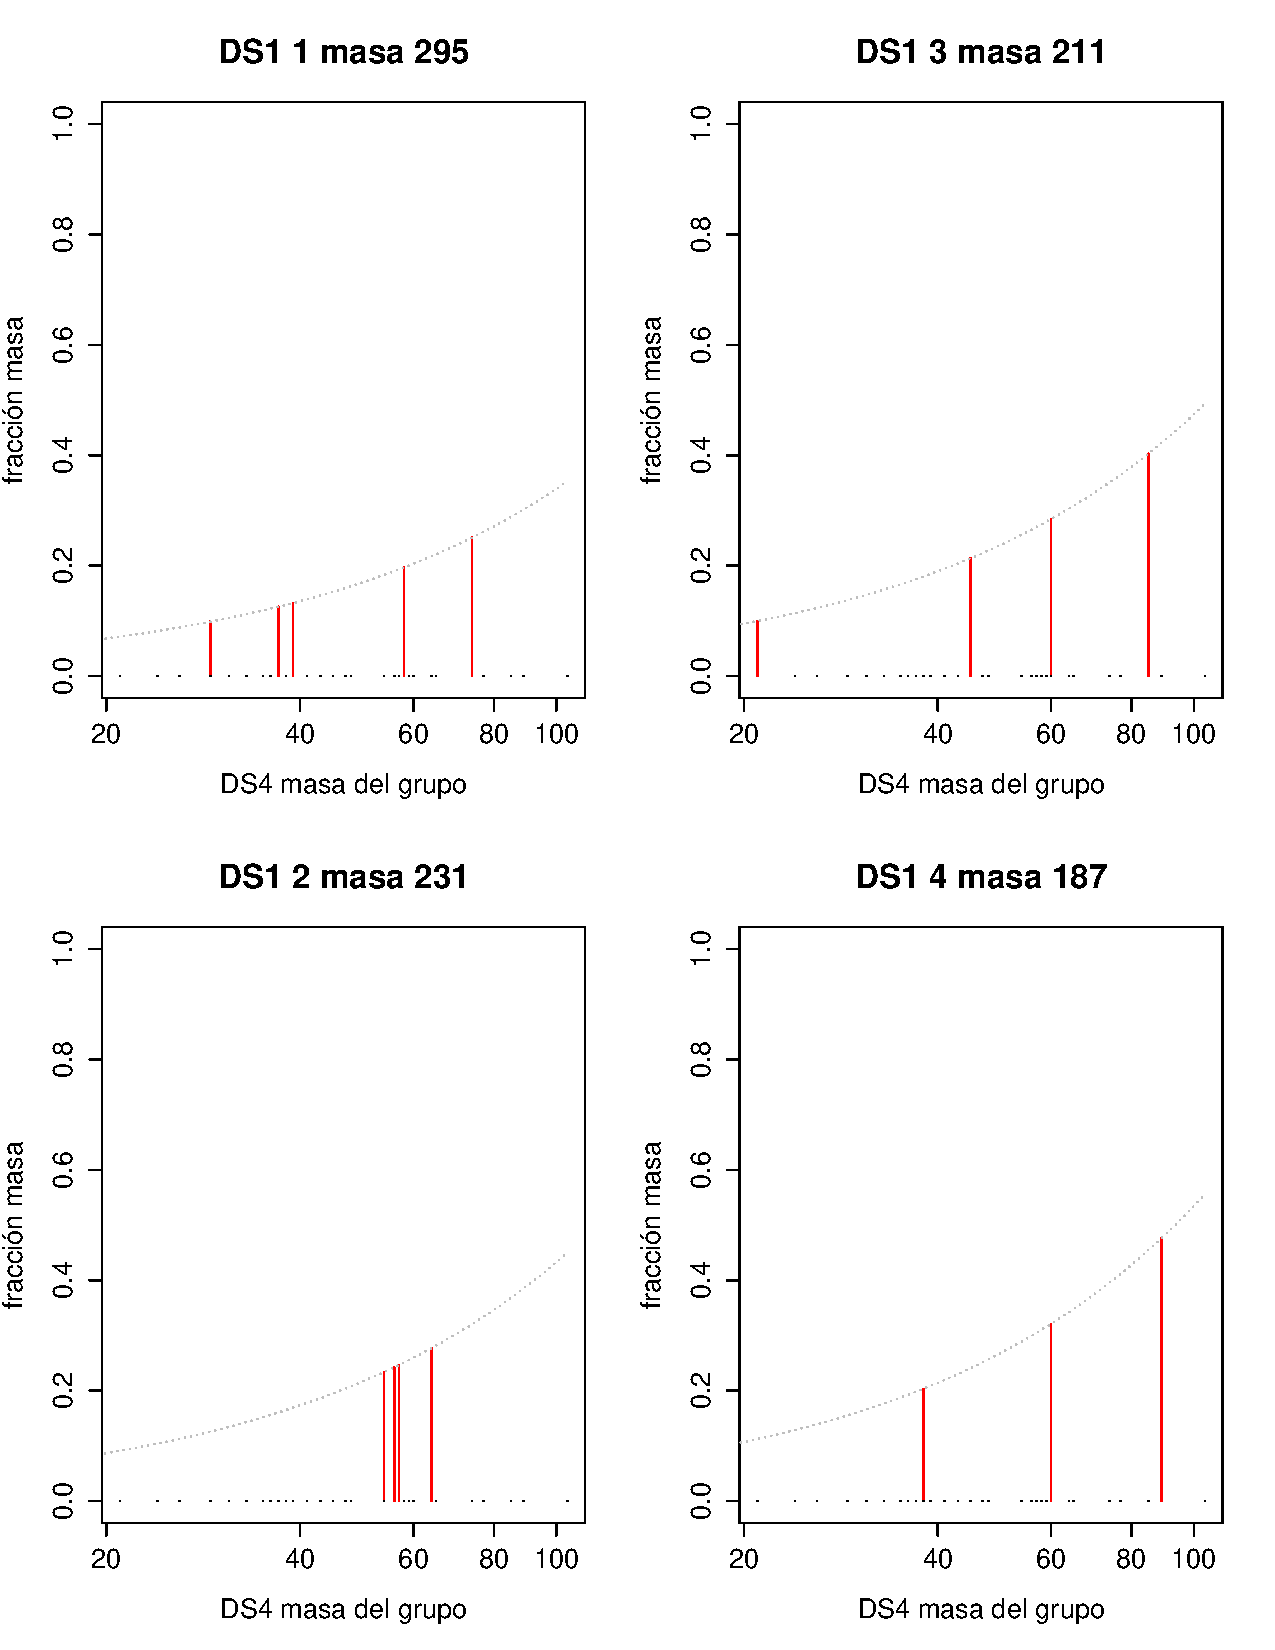
\includegraphics[width=1\textwidth]{fraccion_de_ds1_en_ds4.pdf}
 %   \caption{Fracción de grupos de $ds4$ en los grupos más masivos de $ds1$.}
 %   \label{fig:fraccion_de_ds1_en_ds4}
 %   \end{subfigure}
%    \caption{Fracción de grupos de una partición más fina dentro de grupos en una partición más gruesa para el tratamiento 'Frío', con $ds1$, $ds4$ y k-means. En rojo, aquellos subgrupos que están contenidos en más de un 50\% en el grupo. La linea punteada marca el porcentaje del grupo que representa el total del subgrupo.}
%\end{figure*}

Aquellos subgrupos (los grupos de una partición contenidos en el grupo de otra partición) que están contenidos en más (menos) de un 50\% en el grupo aparecen en rojo (negro). La linea punteada indica el porcentaje del grupo que representaría el subgrupo, si el subgrupo estuviera contenido completamente en el grupo.
En cada caso, se observa que los grupos más grandes de una partición con menor granularidad se parten en grupos más pequeños en otra partición con mayor granularidad, es decir, la partición $ds4$ está contenida en la partición $ds1$ (es un refinamiento de la misma) y esta a su vez está contenida en la partición k-means.\\\\
\clearpage
\section{Discusión}
En el presente análisis de estructura de los grupos obtenidos por medio de los métodos k-means, $ds1$ y $ds4$, encontramos que todos los métodos producen particiones altamente coherentes, con el método k-means generando las particiones más gruesas y los métodos subsiguientes, refinamientos de las mismas. La alta coherencia detectada es indicativo de que cada método logra  hallar estructuras en el espacio de expresión génica. Sin embargo, anticipamos que la interpretación biológica de agrupamientos que contienen centenas de genes puede ser una tarea sumamente dificultosa y no siempre posible. En los siguientes capítulos introduciremos algunas herramientas que nos permitirán cuantificar la homogeneidad biológica de las particiones para encontrar la escala óptima en el análisis de expresión.